\documentclass[a4paper, oneside]{article}
\usepackage[utf8]{inputenc}
\usepackage[ngerman]{babel}
\usepackage[top=2.5cm, bottom=3cm, outer=2.5cm, inner=2.5cm, heightrounded]{geometry}
\usepackage{graphicx}
\usepackage{morefloats}
\usepackage{wrapfig}
\usepackage{hyperref}
\usepackage{cite}
\usepackage{siunitx}
\usepackage[default]{sourcesanspro}
\usepackage[T1]{fontenc}
\usepackage{url}
\usepackage{marginnote}
\usepackage[font=footnotesize]{caption}
\usepackage{color}
\usepackage{xcolor}
\usepackage{multicol}
\usepackage[fleqn]{mathtools}
\usepackage{amssymb}
\usepackage{wrapfig}
\usepackage[noindentafter]{titlesec}
\usepackage{fancyhdr}
\usepackage{lastpage}
\usepackage{comment}

%% LÖSUNGEN ANZEIGEN
\newif\ifshow
%\showtrue
\showfalse

%%%SECTIONING
\renewcommand*{\marginfont}{\noindent\rule{0pt}{0.7\baselineskip}\footnotesize}

\newcommand{\aufgabe}[1]{\subsection{#1}}
\newcommand{\loesung}[1]{\subsubsection{#1}}

\newcommand{\simpleset}[1]{\ensuremath \left\{ #1 \right\}}
\newcommand{\ematrix}[2]{\renewcommand{\arraystretch}{1}\ensuremath\left(\begin{array}{@{}#1@{}}#2\end{array}\right)}

\renewcommand{\theenumi}{\alph{enumi})}
\renewcommand{\labelenumi}{\text{\theenumi}}

\newcounter{aufgabe}
%\newenvironment{lsg}{\loesung}{}
\ifshow
  \newenvironment{lsg}{\loesung}{}
\else
  \excludecomment{lsg}
\fi

\newenvironment{inhalt}
  {\paragraph{Inhalt des Übungsblatts:}\itemize\let\origitem\item}
  {\enditemize\vspace{2em}}

\newcommand{\R}{\ensuremath\mathbb{R}}
\newcommand{\N}{\ensuremath\mathbb{N}}
\newcommand{\Z}{\ensuremath\mathbb{Z}}
\newcommand{\LM}{\ensuremath\mathbb{L}}
\newcommand{\intd}{\ensuremath\mathrm{d}}
\newcommand{\e}{\ensuremath\mathrm{e}}
\renewcommand{\d}{\,\mathrm{d}}
\newcommand{\stf}[1]{\ensuremath \left[ #1 \right]}

\newcommand{\cas}{\hfill (CAS)}
\newcommand{\seite}[1]{\textit{(S. #1)}}

\newcommand{\vektor}[1]{\ensuremath\begin{pmatrix} #1 \end{pmatrix}}


\everymath{\displaystyle}

%Malpunkte
\mathcode`\*="8000
{\catcode`\*\active\gdef*{\cdot}}

%SECTION
\titleformat{\section}
{\clearpage\setcounter{aufgabe}{0}\vspace{1em}\Large\raggedright\bfseries}
{}
{0pt}
{}

\titleformat{\subsection}[runin]
{\stepcounter{aufgabe}\vspace{1px}\normalfont\raggedright\bfseries}
{A\theaufgabe: }
{0pt}
{\ }

\titleformat{\subsubsection}[runin]
{\normalfont\raggedright\bfseries}
{Lösung \theaufgabe: }
{0pt}
{\ }


%FANCYHDR
\pagestyle{fancy}
\lhead{\small Simon König\\ Joshua Fabian}
\rhead{\small Mathecrashkurs 2018}
\cfoot{Seite \thepage\thinspace von\thinspace\pageref{LastPage}}
\lfoot{}
\renewcommand{\headrulewidth}{0.5pt}
\renewcommand{\footrulewidth}{0pt}

\title{Mathe-Crashkurs 2018 - Übungsblatt}
\date{\today}
\author{Simon König, Joshua Fabian}

\chead{\Large Joshua Aufgabensammlung}


\begin{document}



\aufgabe{Winkelberechnung}
\begin{enumerate}
	\item Berechnen Sie die Schnittwinkel der beiden Geraden $g_i$ und $h_i$:
	\begin{itemize}
		\item $g_1: \vec x = \vektor{2\\2\\-3} + r*\vektor{2\\1\\-1}$ und $h_1: \vec x = \vektor{3\\0\\-1} + s* \vektor{1\\-2\\2}$
		\item
	\end{itemize}
	\item
\end{enumerate}

\aufgabe{Lageberechnungen}
\begin{enumerate}
	\item enum
	\item	enum
\end{enumerate}







% IN ÜBUNGSBLATT 4 ANS ENDE?
\aufgabe{Graphanalyse: } (vgl. Abitur 2015)
\begin{multicols}{2}
	Die Abbildung zeigt den Graphen der Ableitungsfunktion $f'$ einer ganzrationalen Funktion $f$.
	Entscheide ob die folgenden Aussagen wahr oder falsch sind. Begründe jeweils Deine Antwort.
	\begin{enumerate}
		\item Der Graph von $f$ hat bei $x=-3$ einen Tiefpunkt.
		\item $f(-2)<f(-1)$
		\item $f''(-2)+f'(-2)<1$
		\item Der Grad der Funktion $f$ ist mindestens vier.
	\end{enumerate}
	\columnbreak

	\centering
	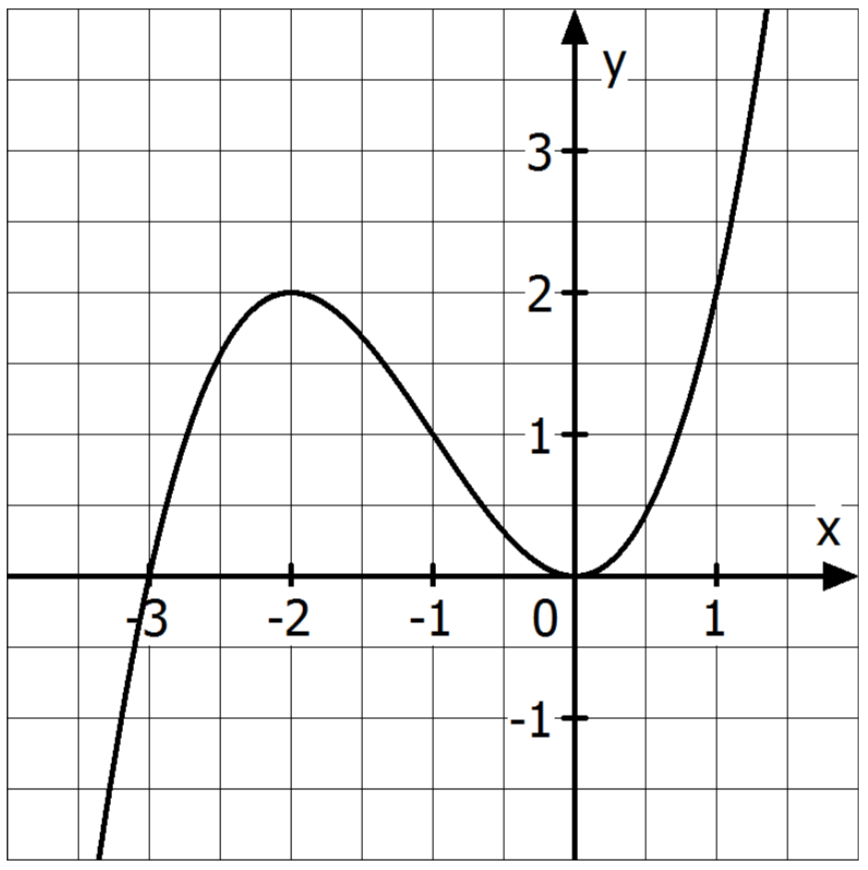
\includegraphics[width=0.7\linewidth]{Graphanalyse.png}
\end{multicols}

\begin{lsg}{}
	\begin{enumerate}
		\item Wahr, Vorzeichenwechsel bei $x=-3$
		\item Wahr, streng monoton steigend im Intervall $[-2;-1]$
		\item Falsch, $f''(-2)+f'(-2)=0+2>1$
		\item Wahr, $f'$ besitzt zwei Extrempunkte $\rightsquigarrow f''$ ist mindestens vom Grad 2. Der Graph der Abbildung könnte auch drei Nullstellen haben, $f'$ ist also mindestens vom Grad 3.
	\end{enumerate}
\end{lsg}



\aufgabe{Extrempunkte}

\begin{lsg}{}

\end{lsg}


\end{document}
